\chapter{Používané metody testování}
V této kapitole se pokusím popsat co nejvíce známích pohledů a způsobů na testování, aby bylo dále možné vybírat, aplikovat a navrhovat testovací systém s ohledem na dnešní metody a trendy v testování. Nejdříve budou popsány úrovně testování, kterými by měl daný výrobek projít, dále popíši způsoby jak testování může probíhat. V poslední kapitole jsou popsány další možné pohledy a přístupy k testování.

\section{Úrovně testování}
Testování výrobků prochází několika stupněmi testování. Některé stupně jsou při vývoji používány bez toho aby jsi to vývojáři uvědomily a některé zase stupně testování zase často opomíjeny. Mnou rozebíráný model má celkem 5 stupňů testování.  Jednotlivé stupně dále popíši a rozeberu jejich přínos a možnosti použití v testovací systému.

\begin{figure}[h]
  \centering
  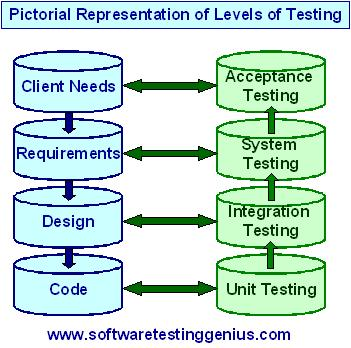
\includegraphics[width=.6\LW]{leveltest}
  \caption{Schéma testovacího modelu}
  \label{fig:leveltest}
\end{figure}

\subsection{Testování programátorem (Developer testing)}
První a úplně nezbytnou částí testování by měl provádět programátoři. Programátor by si měl zkontrolovat jestli je možné firmware přeložit a dále jestli jeho nová či opravená funkcionalita funguje správně. V další fázi tohoto testování by měl otestovat kód jiný programátor, který kód nepsal. Tuto fázi většinou provádí správce projektu při zařazování nové či upravené funkce do hlavní větve repozitáře. Všechny chyby odchycené v této fázi testování ušetří spoustu času stráveném v dalších fázích testování.

Testováním programátorem může vypadat jako samozřejmná věc o která by nemusela být ani uváděna. Bohužel opak je pravdou a i tato situace nástává. Sám jsem byl svědkem situace, kdy lehkovážným přístupem kontroli svých úprav bylo ztraceno spousta času tráveným hledáním spousty lehce vygenerováných chyb.

\subsection{Testování jednotek (Unit testing)}
Úroveň testování jednotek obsahuje testování jednotlvých jednotek software. Jako jednotku lze uvažovat objekt s jednou jedinou funkcionalitou například třídu, objekt, program či softwarový modul. Touto úroveňí testování testujeme správnost zdrojového kódu a ne funkci celého programu. Velmi známým příkladem jsou JUnit testy v javě, kde ke každé třídě a metodě je psán i její test.

Tyto testy je výhodné použít při tvorbě nového projektu, jelikož s unit testy je potřeba počítat již při návrhu zdrojového kódu a při tomto návrhu zároveň tyto testy psát. Dopisování testů do již existujícího projektu by stálo příliš velkou námahu a mnoho úprav kódu pro přizpůsobevání samotného programu pro unit testování.

Jelikož zdrojový kód pro výrobky testované navrhovaným testovacím sytémem jsou vyvýjeny již 10 let a na těchto zdrojových kódech jsou stavěny i nové výrobky. Navíc přes devadesát procent firmwaru používá opensource řešení. Díky těmto skutečnostem je dáno že bude nereálně přidat unit testování do navrhovaného testovacího schématu.

\subsection{Integrační testování (Integration testing)}
Po předchozích dvou úrovních testování, které provádí programátoři přichází fáze kdy se hotový výrobek dostává do ruky testerům. Testeři většinou provádí dvě úrovně testování integrační testování a systémové testování. Někdy jsou tyto dvě fáze spojovány do jedné fáze nazývající se systémově integrační testování. Obě úrovně budou dále detailněji popsány.

Integračním testováním testujeme integraci jednotlivých komponent mezi ostatní komponenty ale také integraci jednotlivých komponent do operačního systému a na konkrétní hardware. Napříkald testování odesíláni sms zpráv na operačním systému Linux běžícím na hardweru konkrétního routeru. Zde je vidět že netestujeme pouze odesílání sms zpráv, ale tuto komponentu v závislosti na operačním systému a hardweru. Jednotlivé komponenty mohou být například subsystémy, databázové implementace, infrastruktura, rozhraní a systémové konfigurace. Integrační testování lze z testování vypustit, jelikož chyby nalezené v této fázi by byly odhaleny ve fázi systémového testování.

\begin{figure}[h]
  \centering
  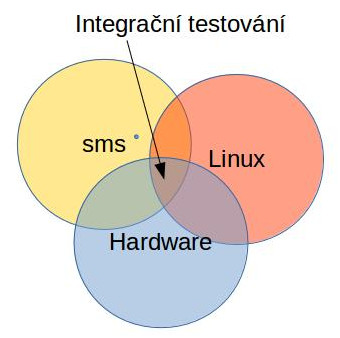
\includegraphics[width=.4\LW]{test_integration}
  \caption{Grafické znázornění integračního testování}
  \label{fig:test_integration}
\end{figure}

Integrační testy již navrhují testerři na základě čtyř základních skutečností. Softwérový a systémový design výrobku, architekturu firmwaru, pracovního postupu s danou komponentou a možnými případy použití. Na základě těchto skutčností tester navrhne testovací příady a postupy. Podle těchto postupů jsou jednotlivé komponenty dále testovány ať již testery či automaticky automatem.

Testovací automat by měl v prvním kroku testovat integračnímy testy všechny základní komponenty routeru jako například posílání sms zpráv, či smnpt klient vůči operačnímu systému Linux či uCLinux, běžícím na každém z 50 různých výrobků podporujících testovanou funkcionalitu. Zde je nejlépe vidět přínos testovacího automatu. Ve skutečnosti by tester měl provést test všech funkcionalit na všech padesáti odlišných výrobcích což je časově nemožné. Zatímco automat tento test může provést každý den na všech výrobcích paralérně během chvilky a tím je ověřena integrace daného programu na všech výrobcích a neunikne žádná chyba ať již je způsobena chybou v firmwaru či chybou některé ze součástí routeru jako například bezdrátového modulu.

\subsection{SIT - Systémové testování (System testing)}
Poslední fází testování probíhající ve společnosti vyvýjecí daný produkt je systémové testování. V této fázi se testuje výrobej jako celek z pohledu zákazníka. Jsou navrhnuty jednotlive testovací případy, které mohou či nastavájí v praxi a dle těchto případů jsou výrobky testovány. Jako příklad může být uveden router ke kterému je přes ethernet připojena IP kamera a přes sériové rozhranní senzor. Data z těchto zařízení jsou přes OpenVPN tunel sestavený přes mobilní spojení posílána na vzdálený server.

Systémové testy mohou obsahovat funkční i nefunkční testy. Tyto testy jsou dále popsáné v sekci věnované typech testování. Dále je možné testovat kvalitu a rychlost přenosu dat. Tyto testy jsou prováděny na výrobcích ve stadartním, ale i v stíženém prostředí, například v klimatické komoře nebo v okolí emc vyzařovaní. Dále je možné na systémové testování pohlížet jako na testování bílé či černé skříňky. Oba tyto způsoby jsou také dále popsány v kapitole věnující se této problematice.

V našem případě bude systémové testování prováděno ve stejném kroku jako integrační testování, čili se tento model blíží popisované možnosti spojení systémových a integračních testů. V popisovaném případě někdy lze určit hranici mezi systémovými a integračním testy a někdy je toto rozdělění těžko určit. Většina testů stejně jako integrační testy bude možné provádě automaticky pomocí testovacího automatu. Jiné testy jako napříkald testy v klimatické komoře budou muset být dále prováděny manuálně, jelikož všech padesát výrobků se do klimatické komory nevejde. Na druho stranu tyto testy nezávisí na změně firmwaru, tak se většinou provádí pouze jednou a to při vyvinutí nového výrobku a ne při každé změně firmwaru.

\subsection{UAT - Akceptační testování (Acceptance testing)}
Poslední úrovní testování je akceptační testování. Akceptační testování již není prováděno v testery ve firmě kde je výrobek vyvýjen, ale již přímo u zákazníka. Zákazník testuje výrobek ve své konkrétní aplikaci. Případné chyby či nesrovnalosti jsou reportovány zpět vyvojovému týmu a bývá očekávána rychlá reakce na opravu těchto chyb. Jelikož se tato fáze provádí až u koncového zákazníka tato práce se touto fází nebude dále zabývat.


\section{Testovací procesy}
Jednotlivé fáze testování lze provádět třemi různými způsoby. Všechny tři způsoby se liší hlavně v délce a složitosti návrhu a provádění testů a v neposlední řadě v pokrytí testovacích případů. Podle složitosti návrhu testů by bylo možné popisované způsoby testování seřadit jako testování založené na modelech, automatizované testování a nakonec manuální testování. Rychlostí a efektivitou provádění testů jsou tyto způsoby seřazeny přesně obráceně. Cílem této práce je automatizovat a tím zkrátit provádění testů a zároveň rozšířit možností testování, takže bude pokoušeno o přechod z nynějšího manuálního testování na automatizované testování a v některých částech na testování založené na modelech.

\subsection{Manuální testování}
Prvním 


\subsection{Automatizované testování}
\subsection{Testování založené na modelech}


\section{Typy testování}

\subsection{Instalační testy}
\subsection{Testy splněním a selháním}
\subsection{Progresní a regresní testy}
\subsection{Smoke testy}
\subsection{Funkční a nefunkční testy}
\subsection{Testování bílé a černé skříňky}
\subsection{Statické a dynamické testy}

\section{Modely vývoje a testování}

\endinput
